\clearpage
\subsection{Field Observations}
This section contains outcrop data of a few selected field areas. 
\begin{table}[h!]
\centering
\caption{Unique sedimentary interpretation keywords extracted from field analogue studies.}
\begin{tabular}{|p{4cm}|p{4cm}|p{4cm}|}
\hline
\multicolumn{3}{|c|}{\textbf{Geometries / structures}} \\
\hline
Chaotic bedding & Concave & Continuous \\
Cross-stratification & Deformation & Dipping \\
Discontinuous & Erosion & Cross-bedding \\
Fill deposit & Fine/coarse-grained & Horizontal \\
Horizontal bedding & Irregular & Laminate \\
Laterally stacked & Lenticular & onlap \\
Low angle & Parallel & Planar \\
Ripples & Semi-continuous & Shallow scours \\
Sinuous & Sinusoidal stratification & Tabular \\
Trace fossils & Vertically stacked & Wavy pattern \\
\hline
\end{tabular}
\label{tab:field-keywords}
\end{table}

\subsubsection{Lacustrine}
\begin{figure}[h!]
    \centering
    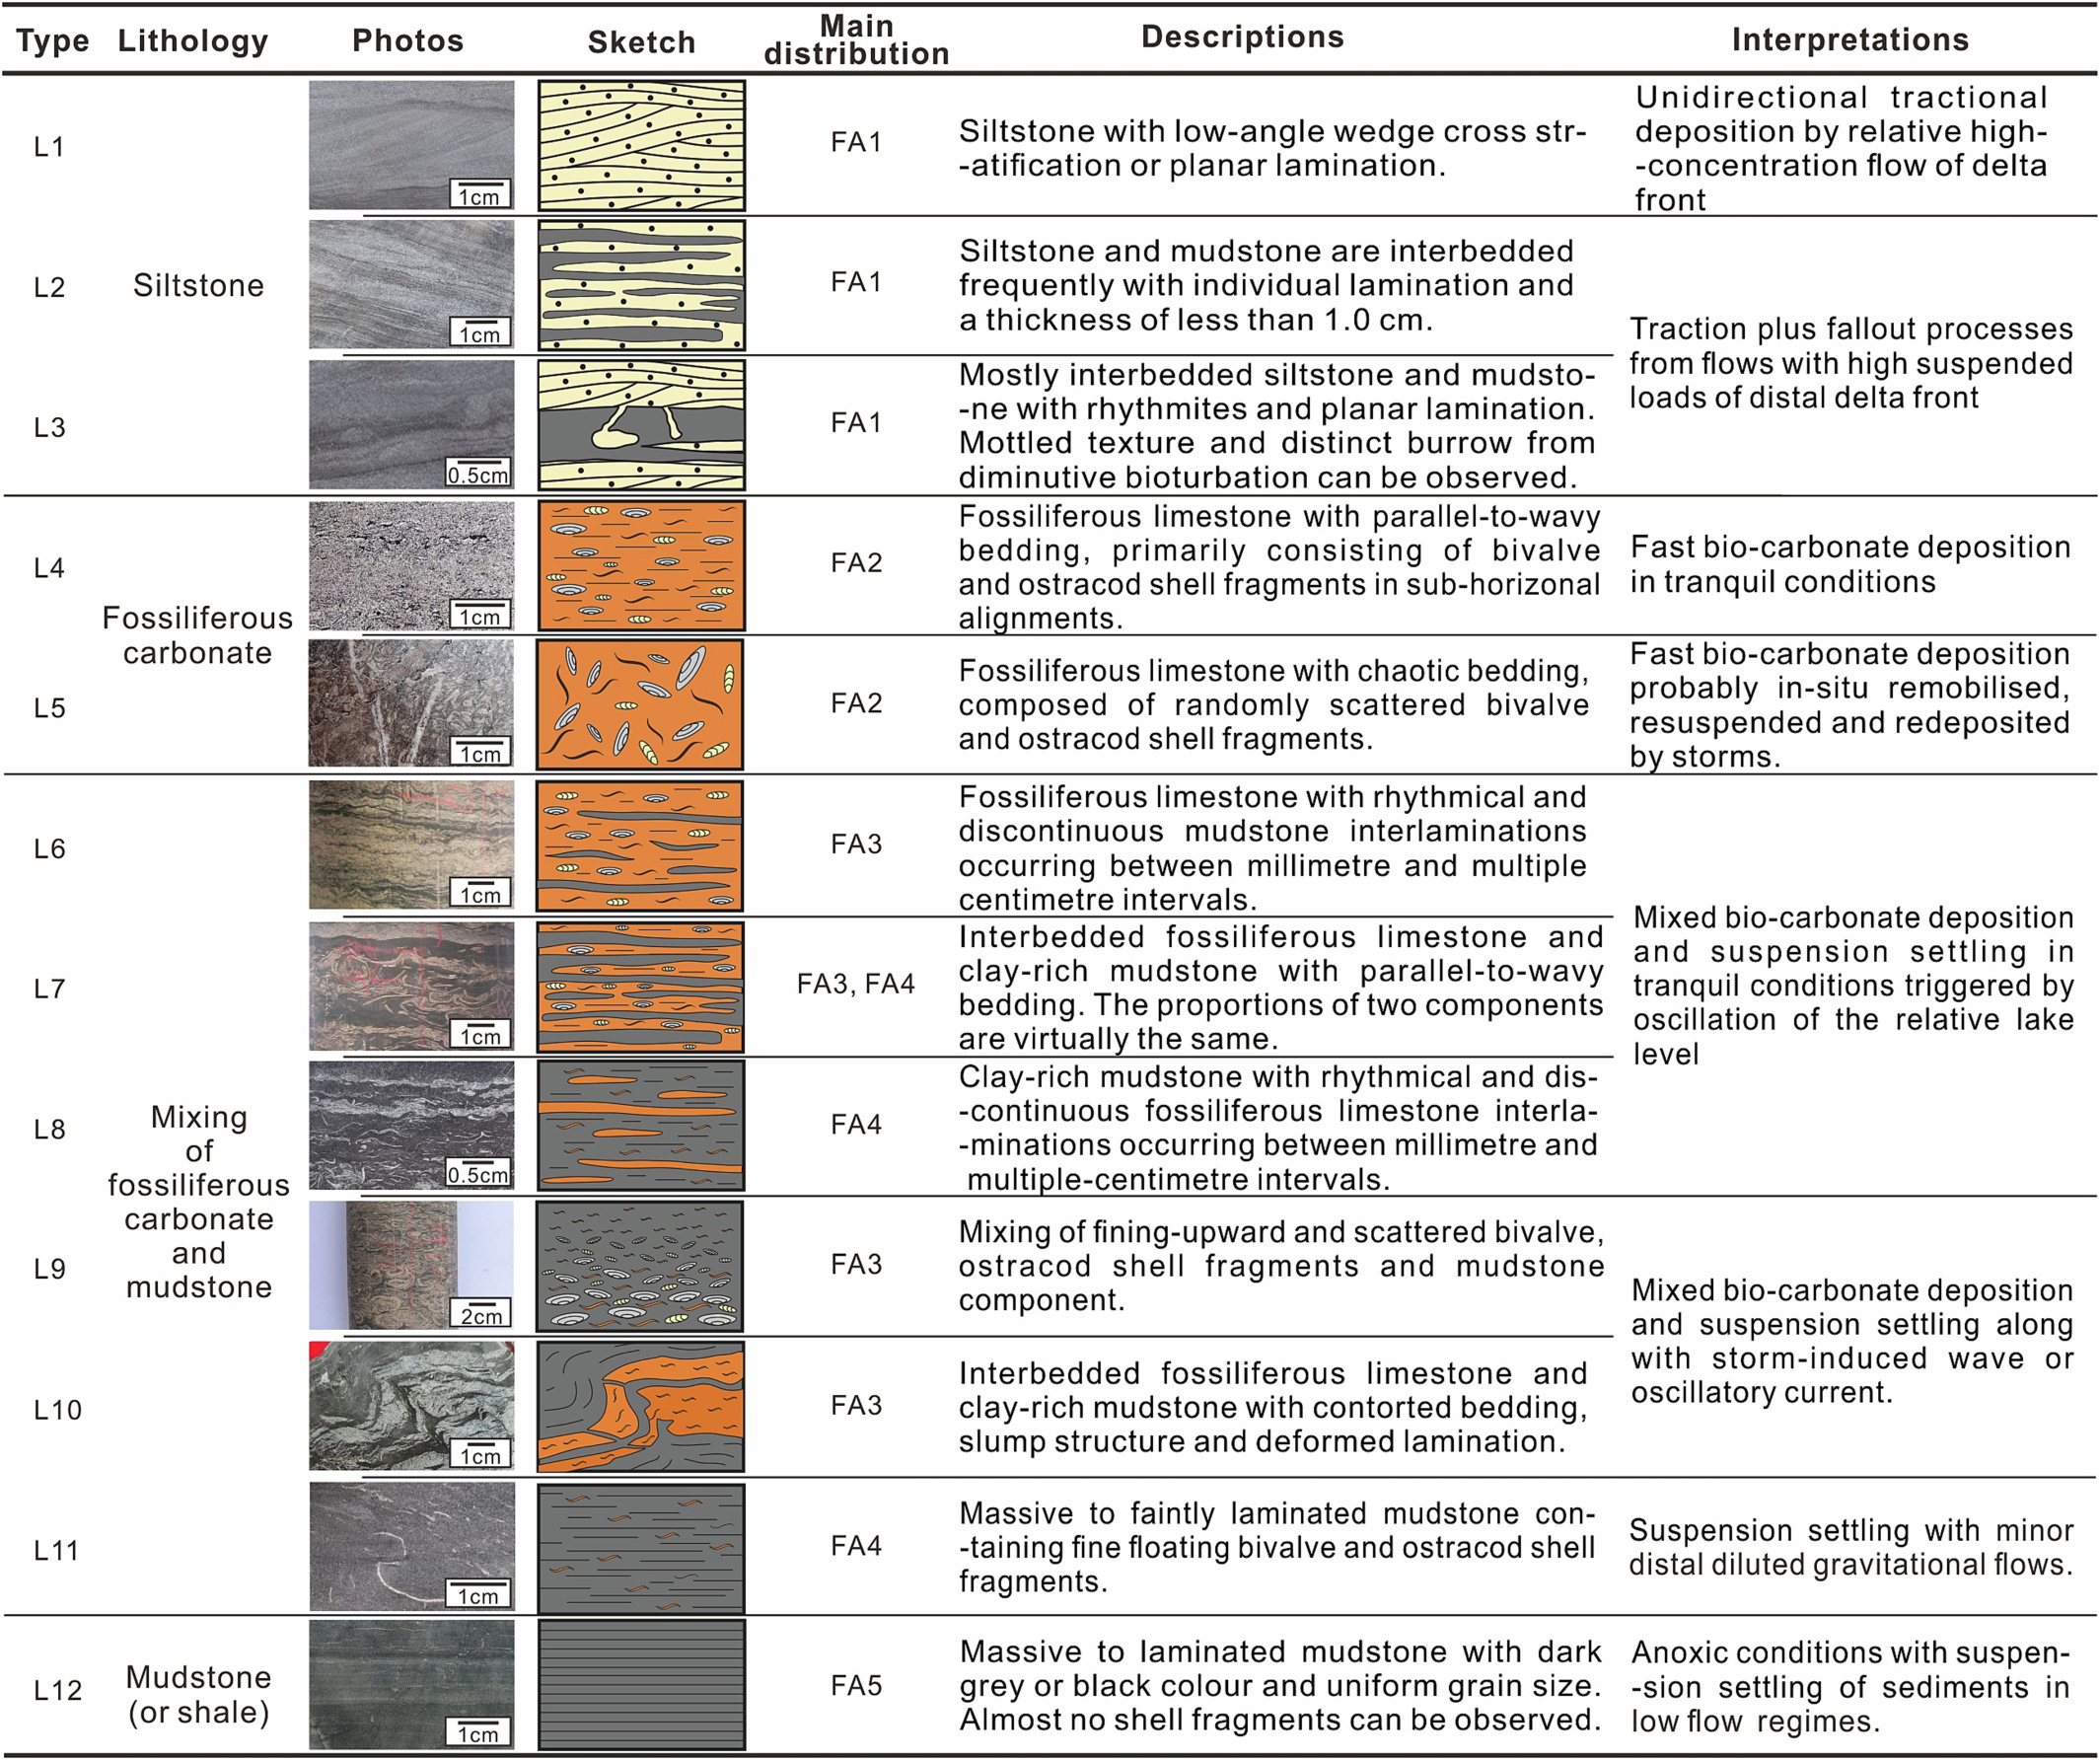
\includegraphics[width=0.75\linewidth]{Figures/0.4Field/Cui2023_trace_field_1.png}
    \caption[Siliciclastic-carbonate lacustrine system]{Siliciclastic-carbonate lacustrine system \citep{Cui2023}. \textbf{Keywords:} low-angle wedge, cross-stratification, planar lamination, parallel, wavy pattern, chaotic bedding, deformation}
    \label{fig:Cui23-1}
\end{figure}
\clearpage

\subsubsection{Fluvial}
\begin{figure}[h!]
    \centering
    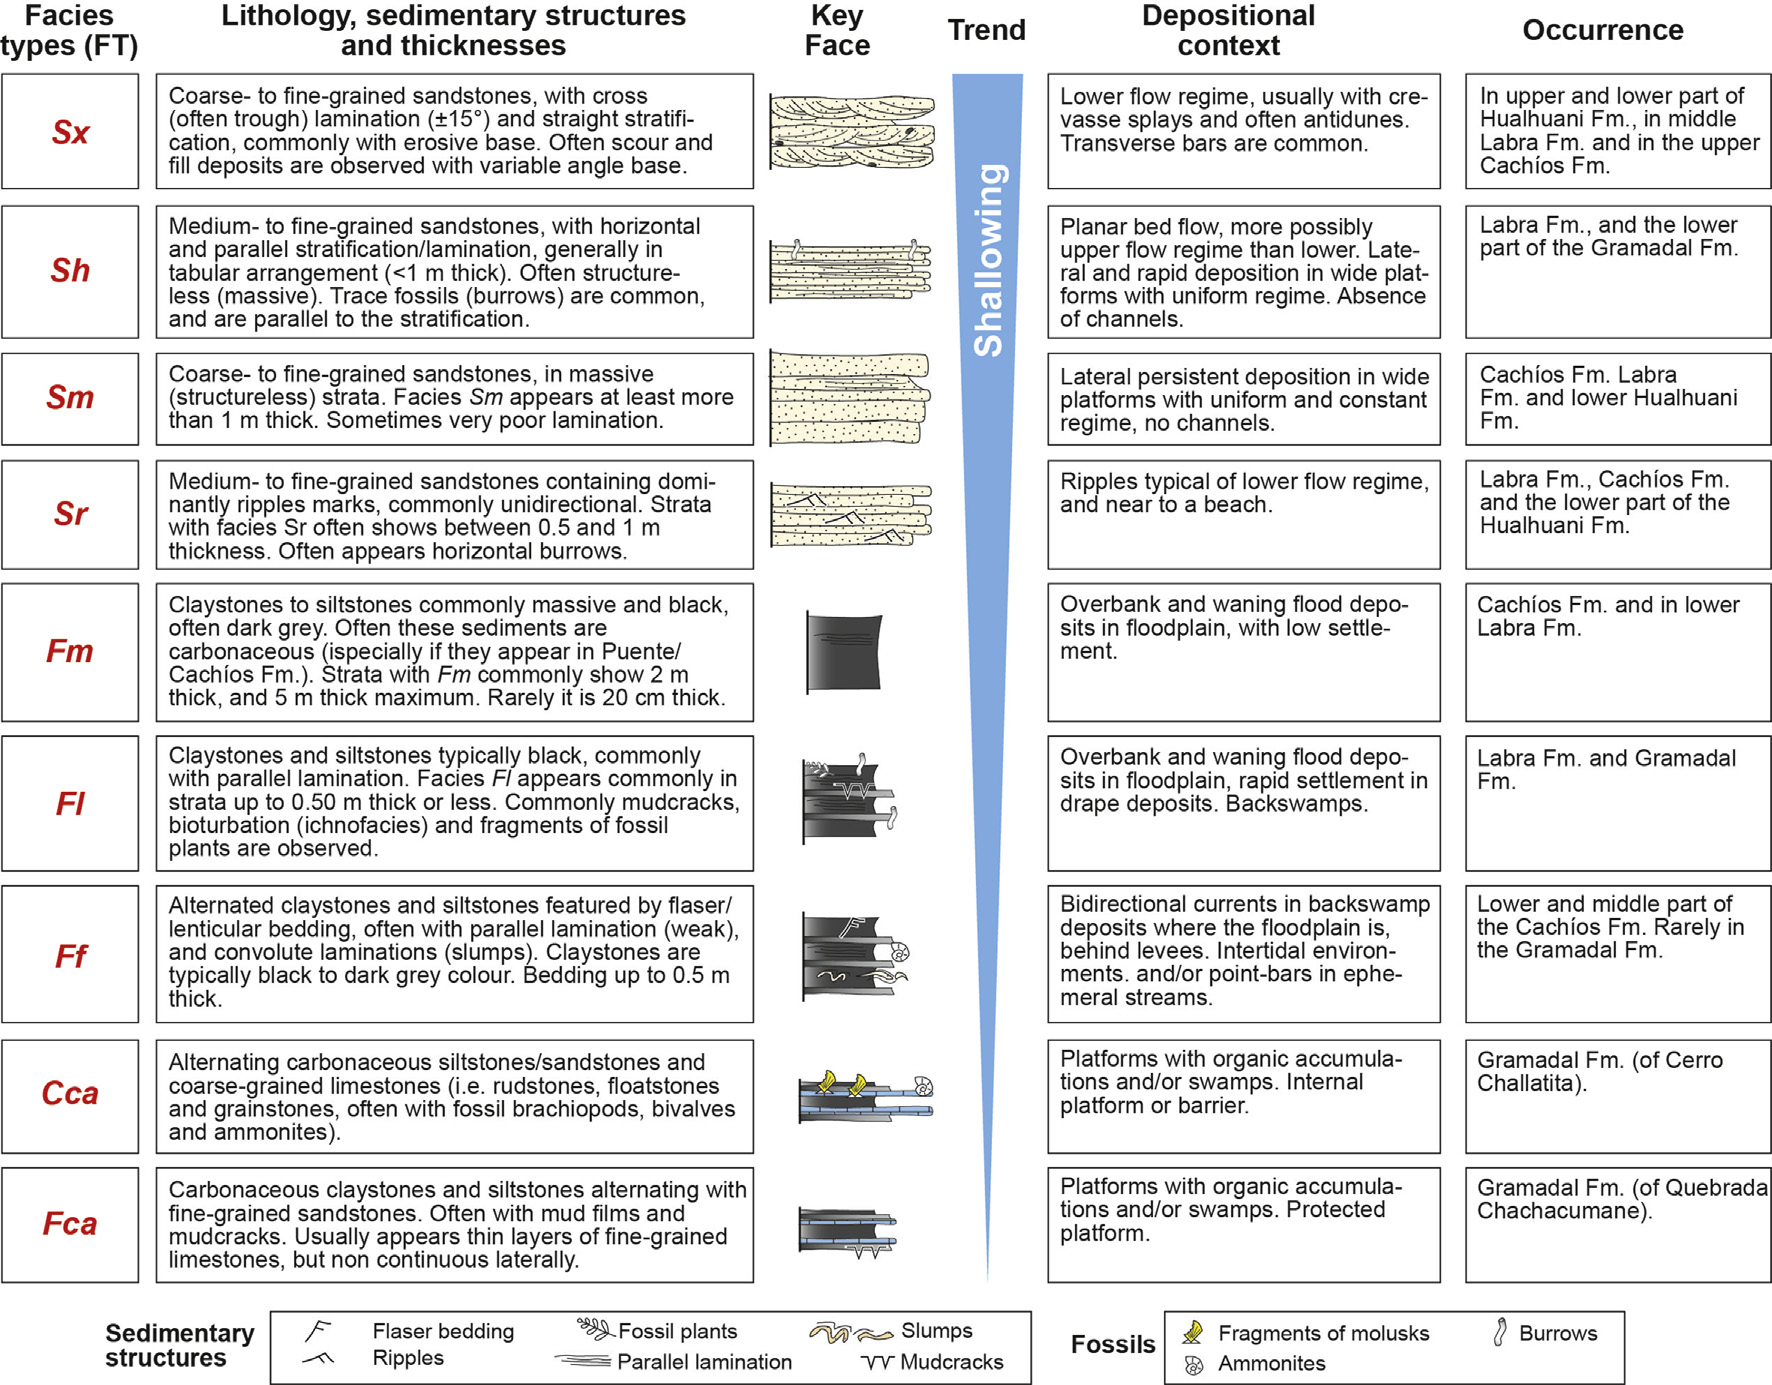
\includegraphics[width=0.75\linewidth]{Figures/0.4Field/Alvan2018_trace_field_1.png}
    \caption[An overview of several Sedimenatry facies]{An overview of several Sedimenatry facies\citep{Alvan2018}. \textbf{Keywords:} Cross lamination, fill deposit, coarse-grained, fine-grained, parallel, lenticular, horizontal layers.}
    \label{fig:Alvan2018-1}
\end{figure}

\begin{figure}[h!]
    \centering
    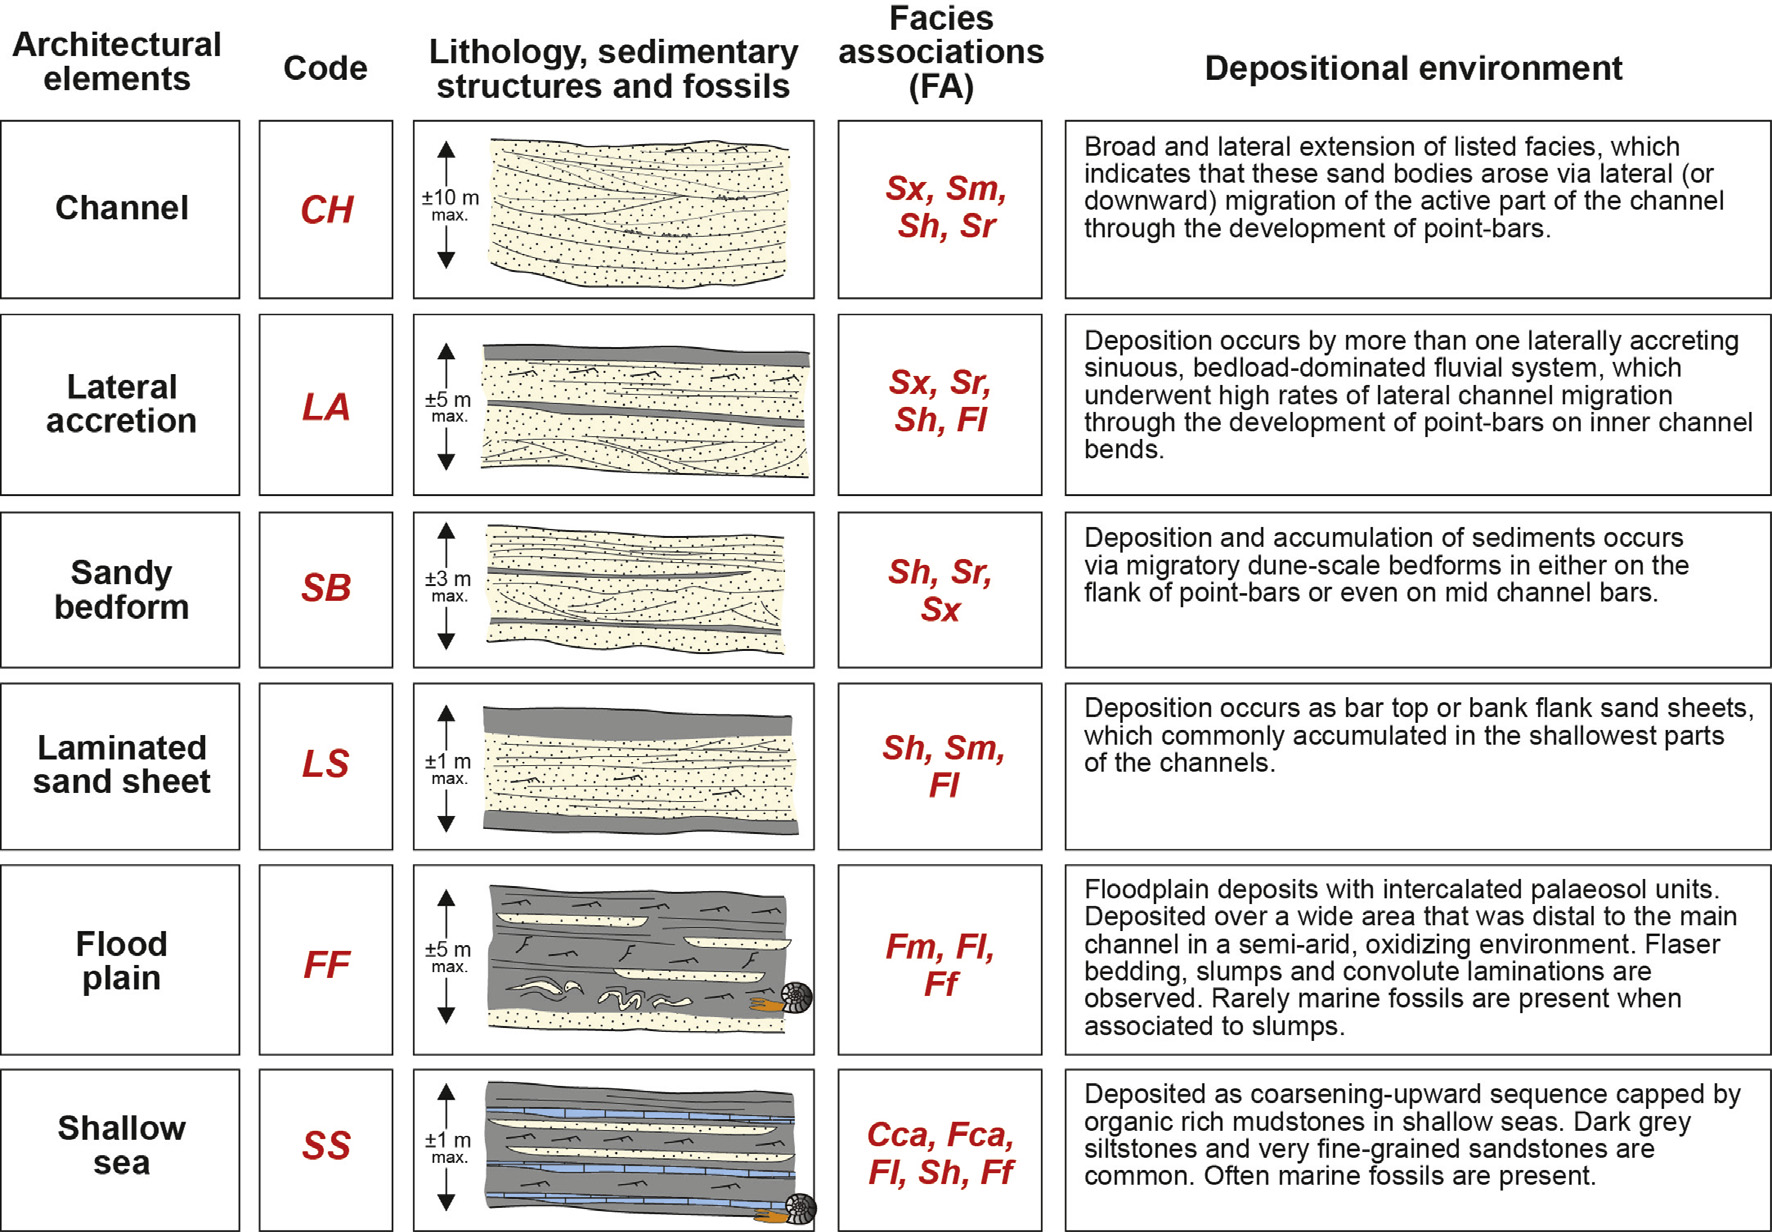
\includegraphics[width=0.75\linewidth]{Figures/0.4Field/Alvan2018_trace_field_2.png}
    \caption[An overview of several Sedimenatry facies]{An overview of several Sedimenatry facies\citep{Alvan2018}. \textbf{Keywords:} Lateral extension, parallel, onlap, downlap, sinuous, cross-bedding.}
    \label{fig:Alvan2018-2}
\end{figure}

\begin{figure}[h!]
    \centering
    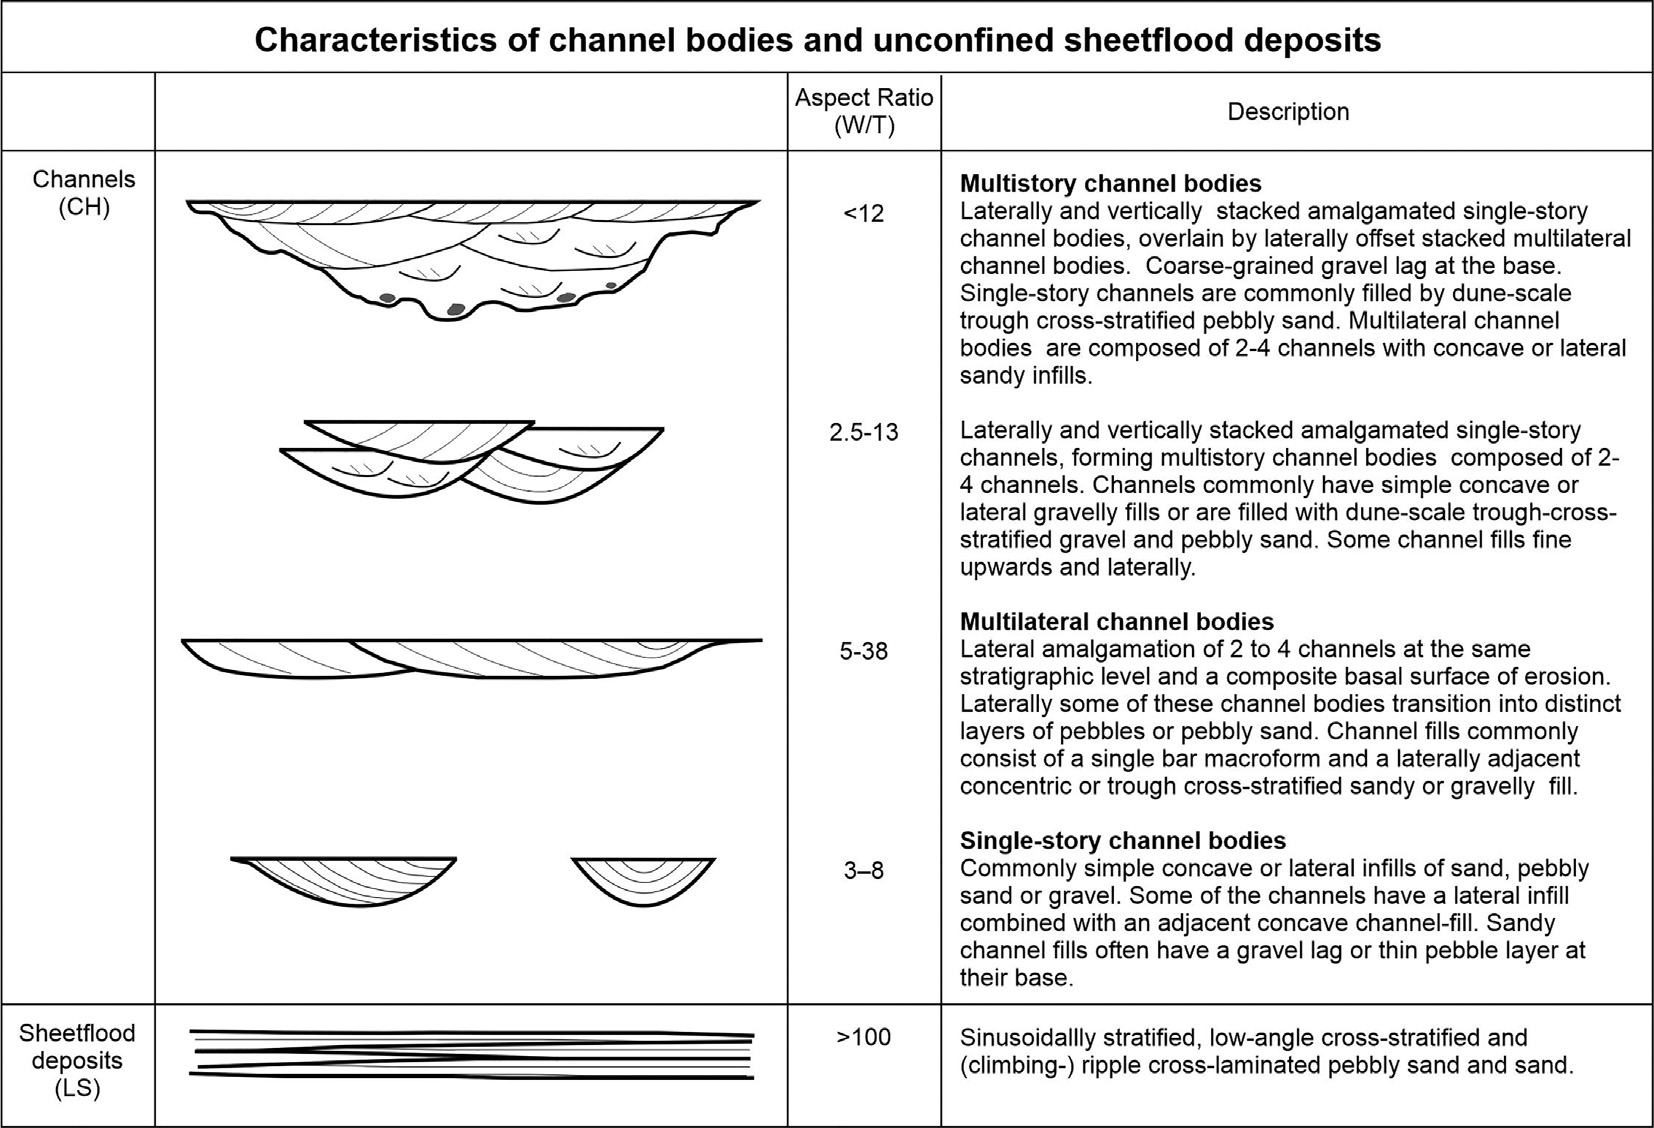
\includegraphics[width=0.75\linewidth]{Figures/0.4Field/Winsemann2022.png}
    \caption[Characteristics of channel bodies and sheetflood deposits]{Characteristics of channel bodies and sheetflood deposits \citep{Winsemann2022}. \textbf{Keywords:} Concave, laterally stacked, vertically stacked, erosional surface, dipping, cross-stratification, sinusoidal stratification, low angle, ripple.}
    \label{fig:Winsemann22-1}
\end{figure}

\begin{figure}[h!]
    \centering
    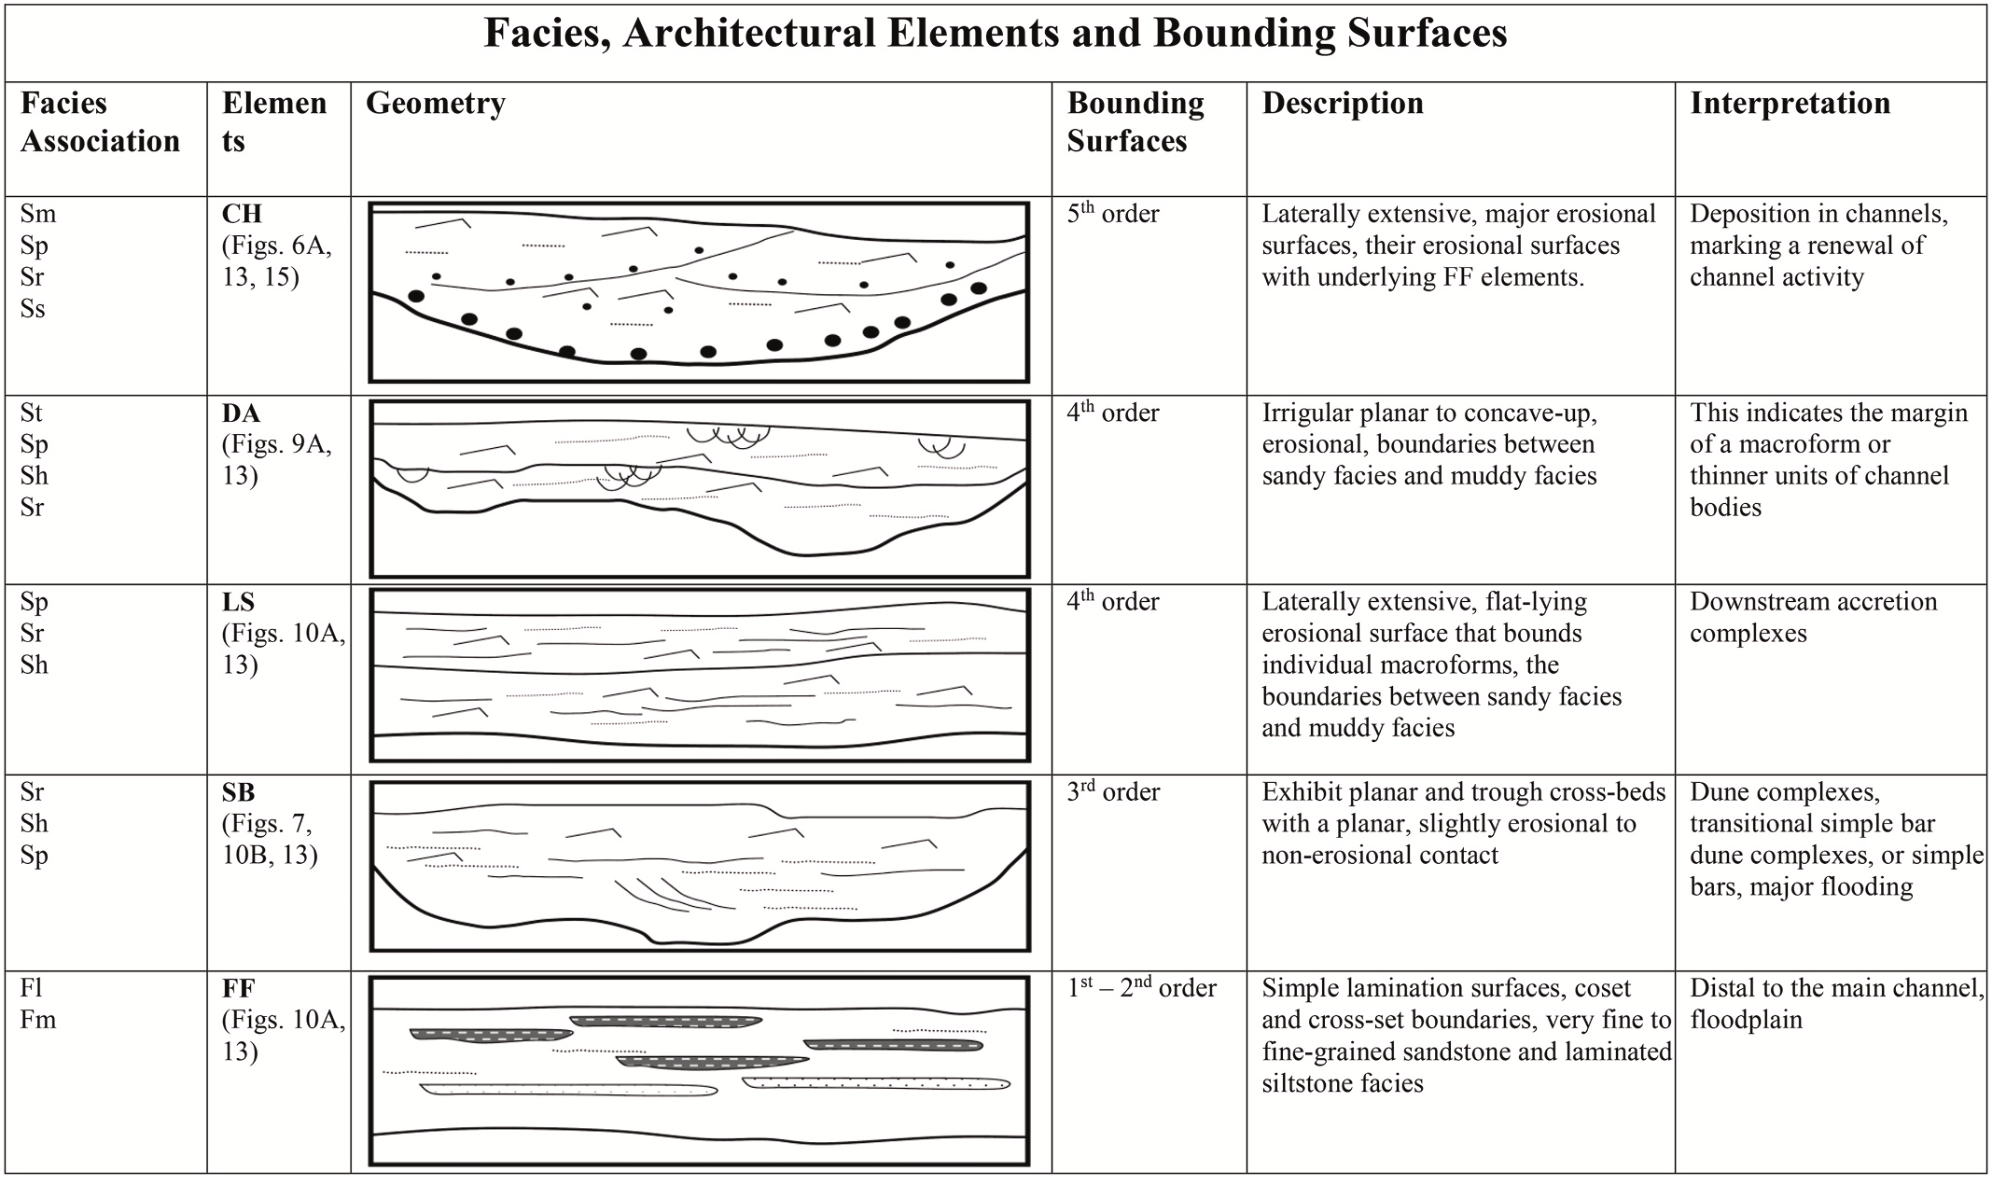
\includegraphics[width=0.75\linewidth]{Figures/0.4Field/Poursoltani2020.png}
    \caption[Summary of architectural elements in a lower sandstone]{Summary of architectural elements in a lower sandstone \citep{Poursoltani2020}. \textbf{Keywords:} Laterally extensive, erosional surface, irregular, concave-up, cross-bedding, horizontal, dipping.}
    \label{fig:Poursoltani20-1}
\end{figure}

\begin{figure}[h!]
    \centering
    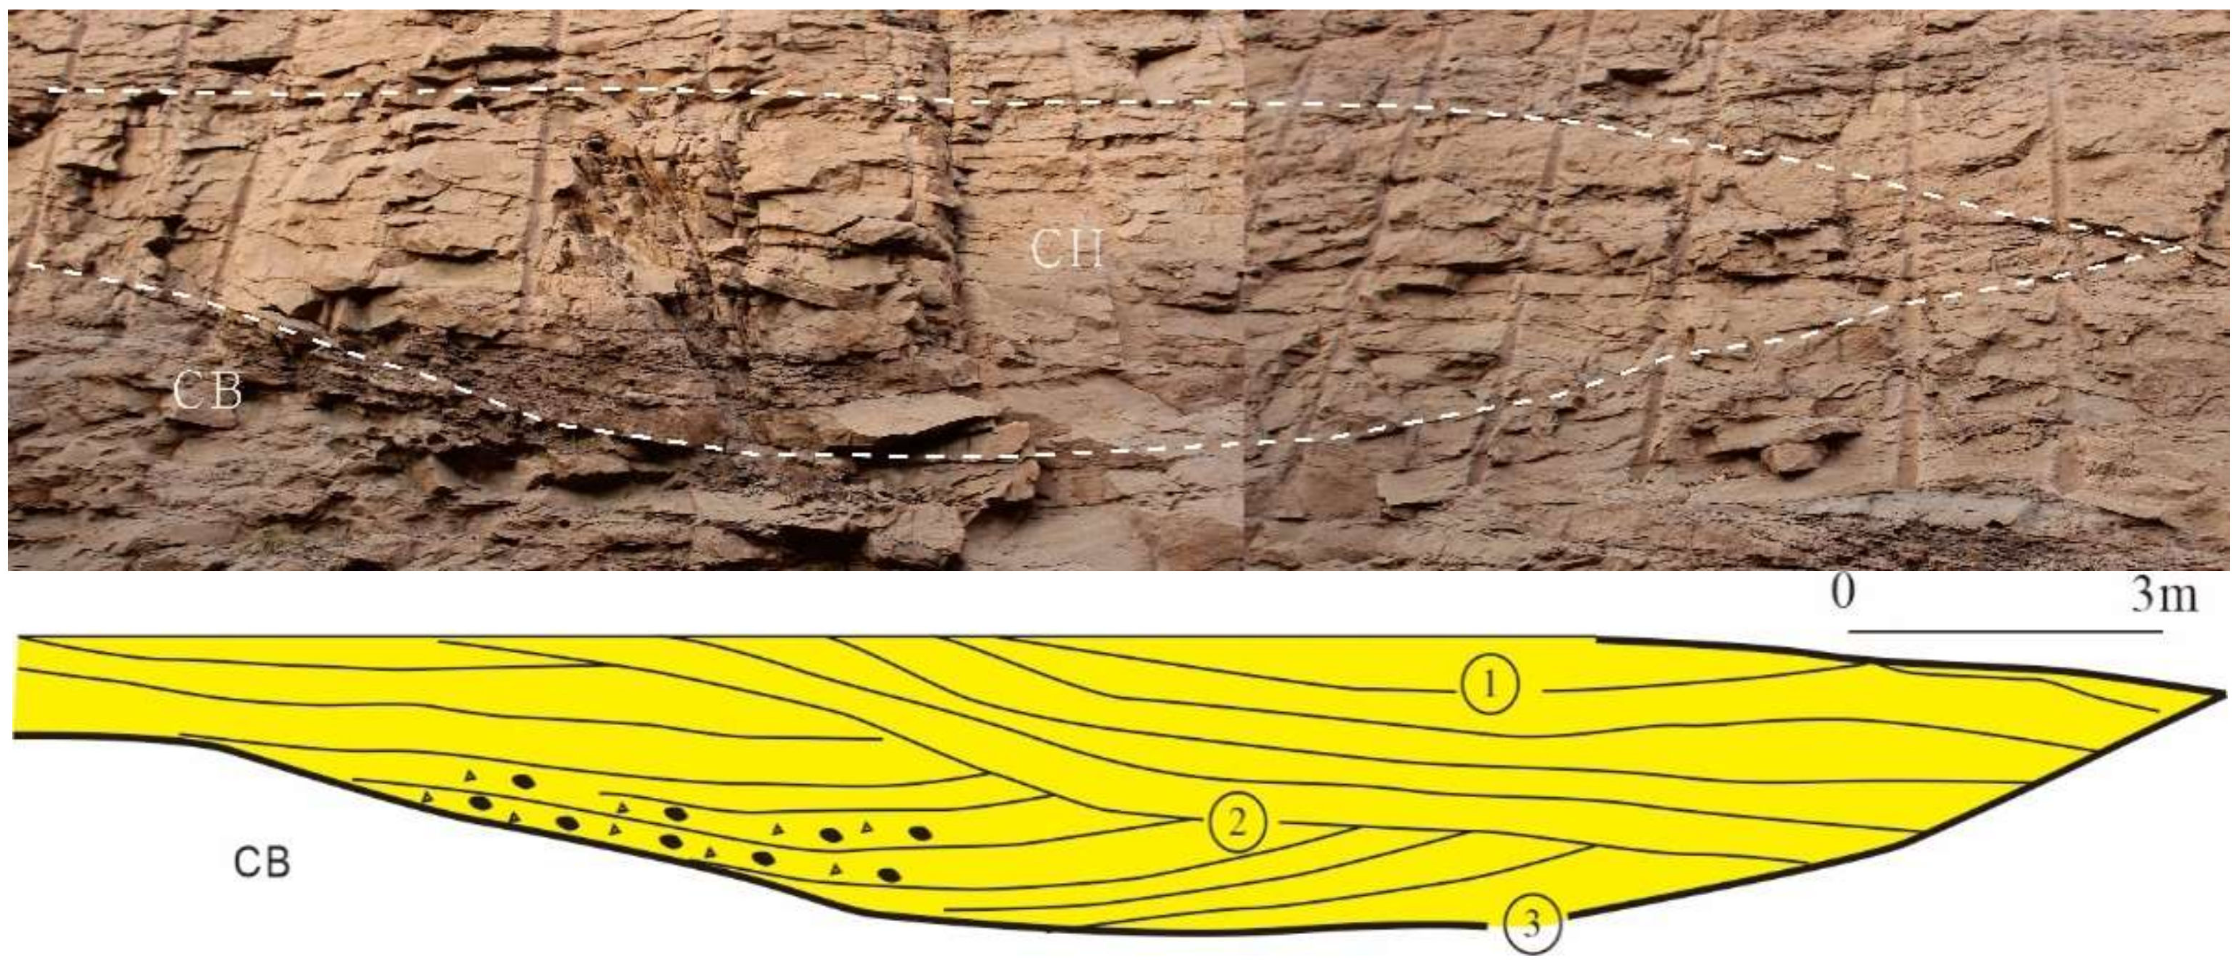
\includegraphics[width=0.75\linewidth]{Figures/0.4Field/Guo2022_2.png}
    \caption[Channel architecture of the outcrop section of the Yungang Formation (1)]{Channel architecture of the outcrop section of the Yungang Formation \citep{Guo2022}. \textbf{Keywords:} Cross-bedding, dipping, onlap, erosion.}
    \label{fig:Guo2022-2}
\end{figure}

\begin{figure}[h!]
    \centering
    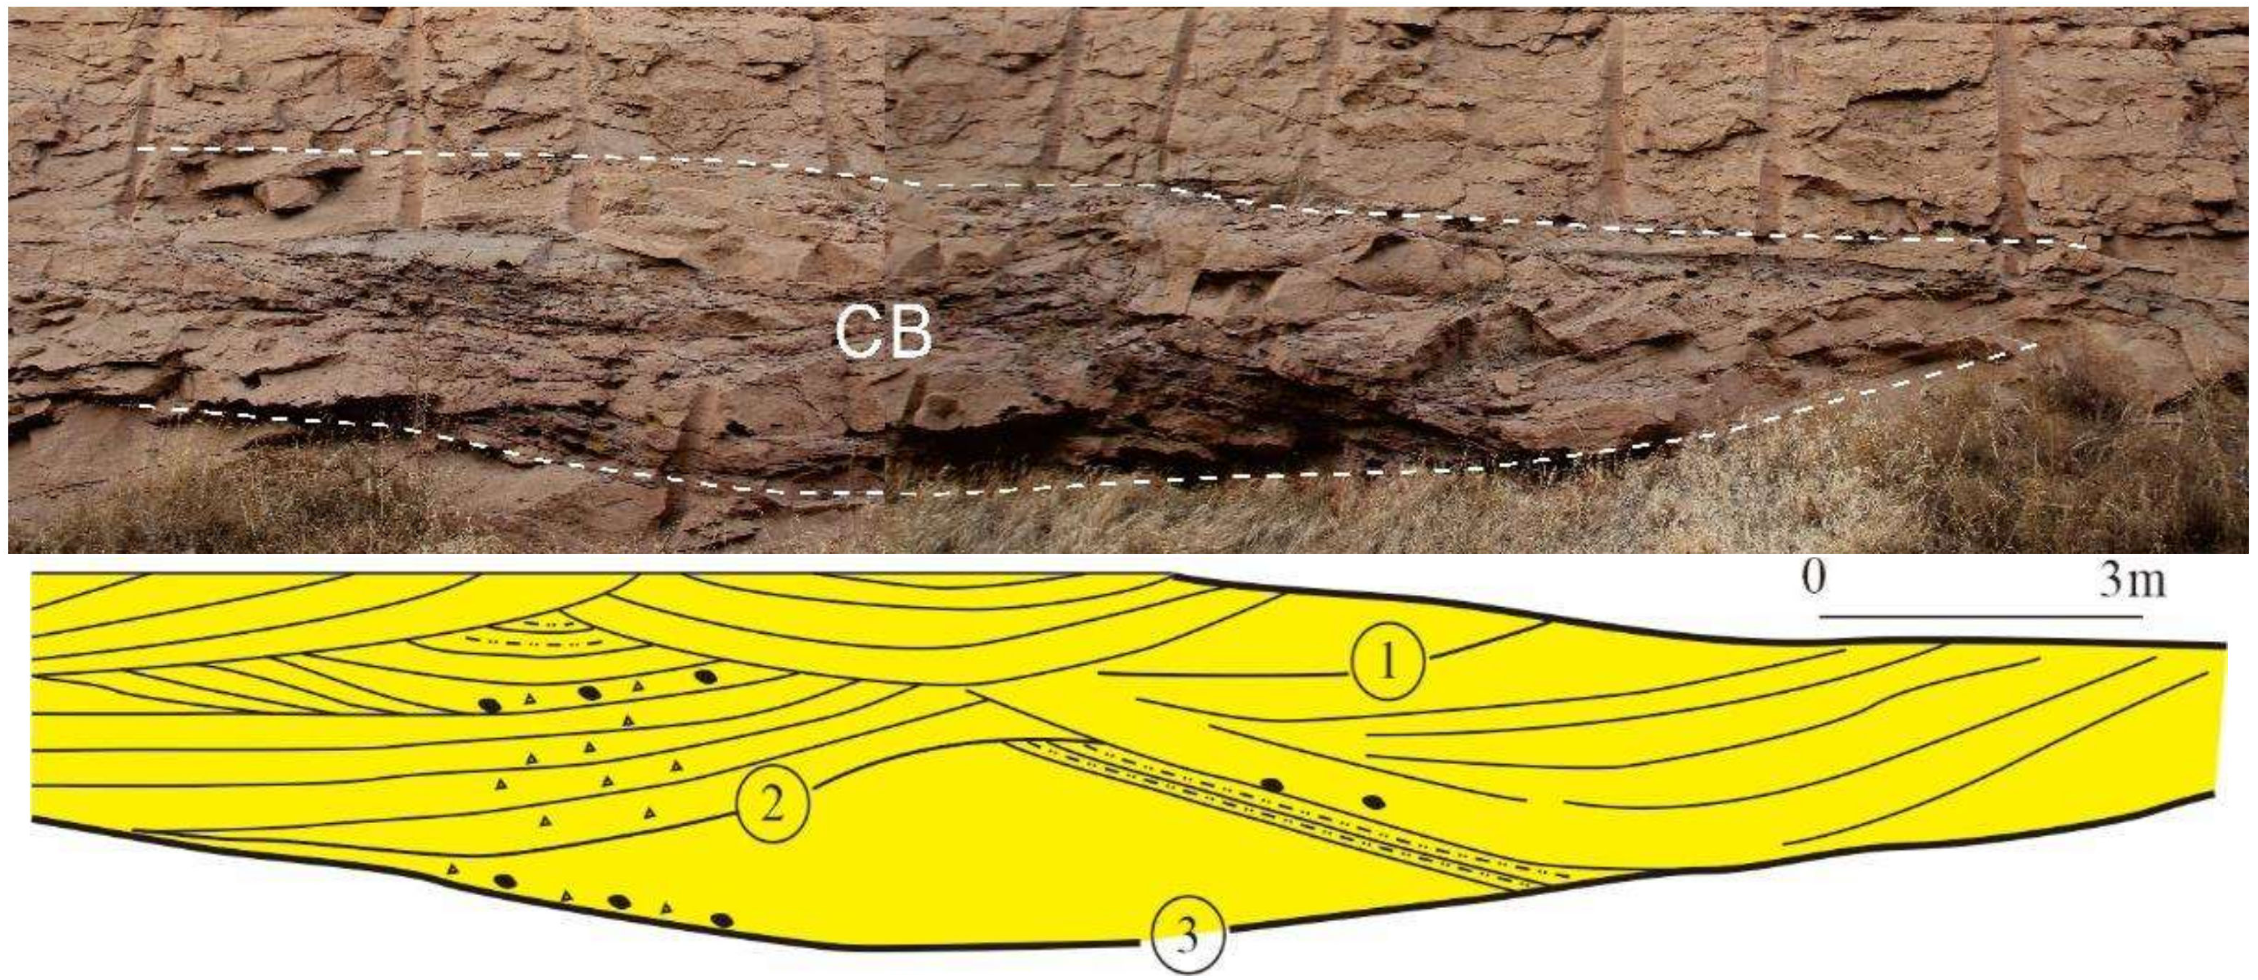
\includegraphics[width=0.75\linewidth]{Figures/0.4Field/Guo2022_3.png}
    \caption[Channel architecture of the outcrop section of the Yungang Formation (2)]{Channel architecture of the outcrop section of the Yungang Formation \citep{Guo2022}. \textbf{Keywords:} Cross-bedding, erosion, dipping, onlap.}
    \label{fig:Guo2022-3}
\end{figure}
\begin{figure}[h!]
    \centering
    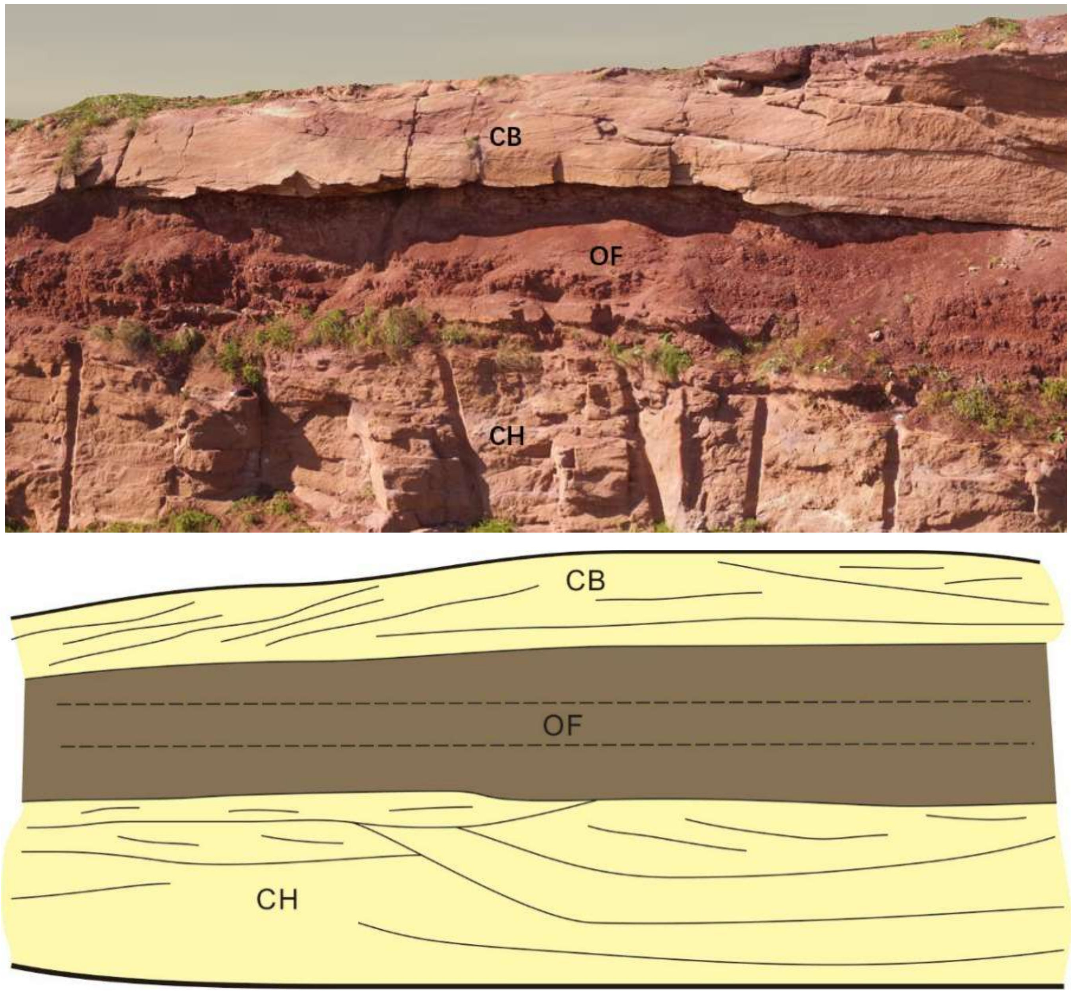
\includegraphics[width=0.75\linewidth]{Figures/0.4Field/Guo2022_4.png}
    \caption[Channel architecture of the outcrop section of the Yungang Formation (3)]{Channel architecture of the outcrop section of the Yungang Formation \citep{Guo2022}. \textbf{Keywords:} Cross-bedding, erosion, dipping, onlap, horizontal layering, semi-continuous, continuous.}
    \label{fig:Guo2022-4}
\end{figure}

\begin{figure}[h!]
    \centering
    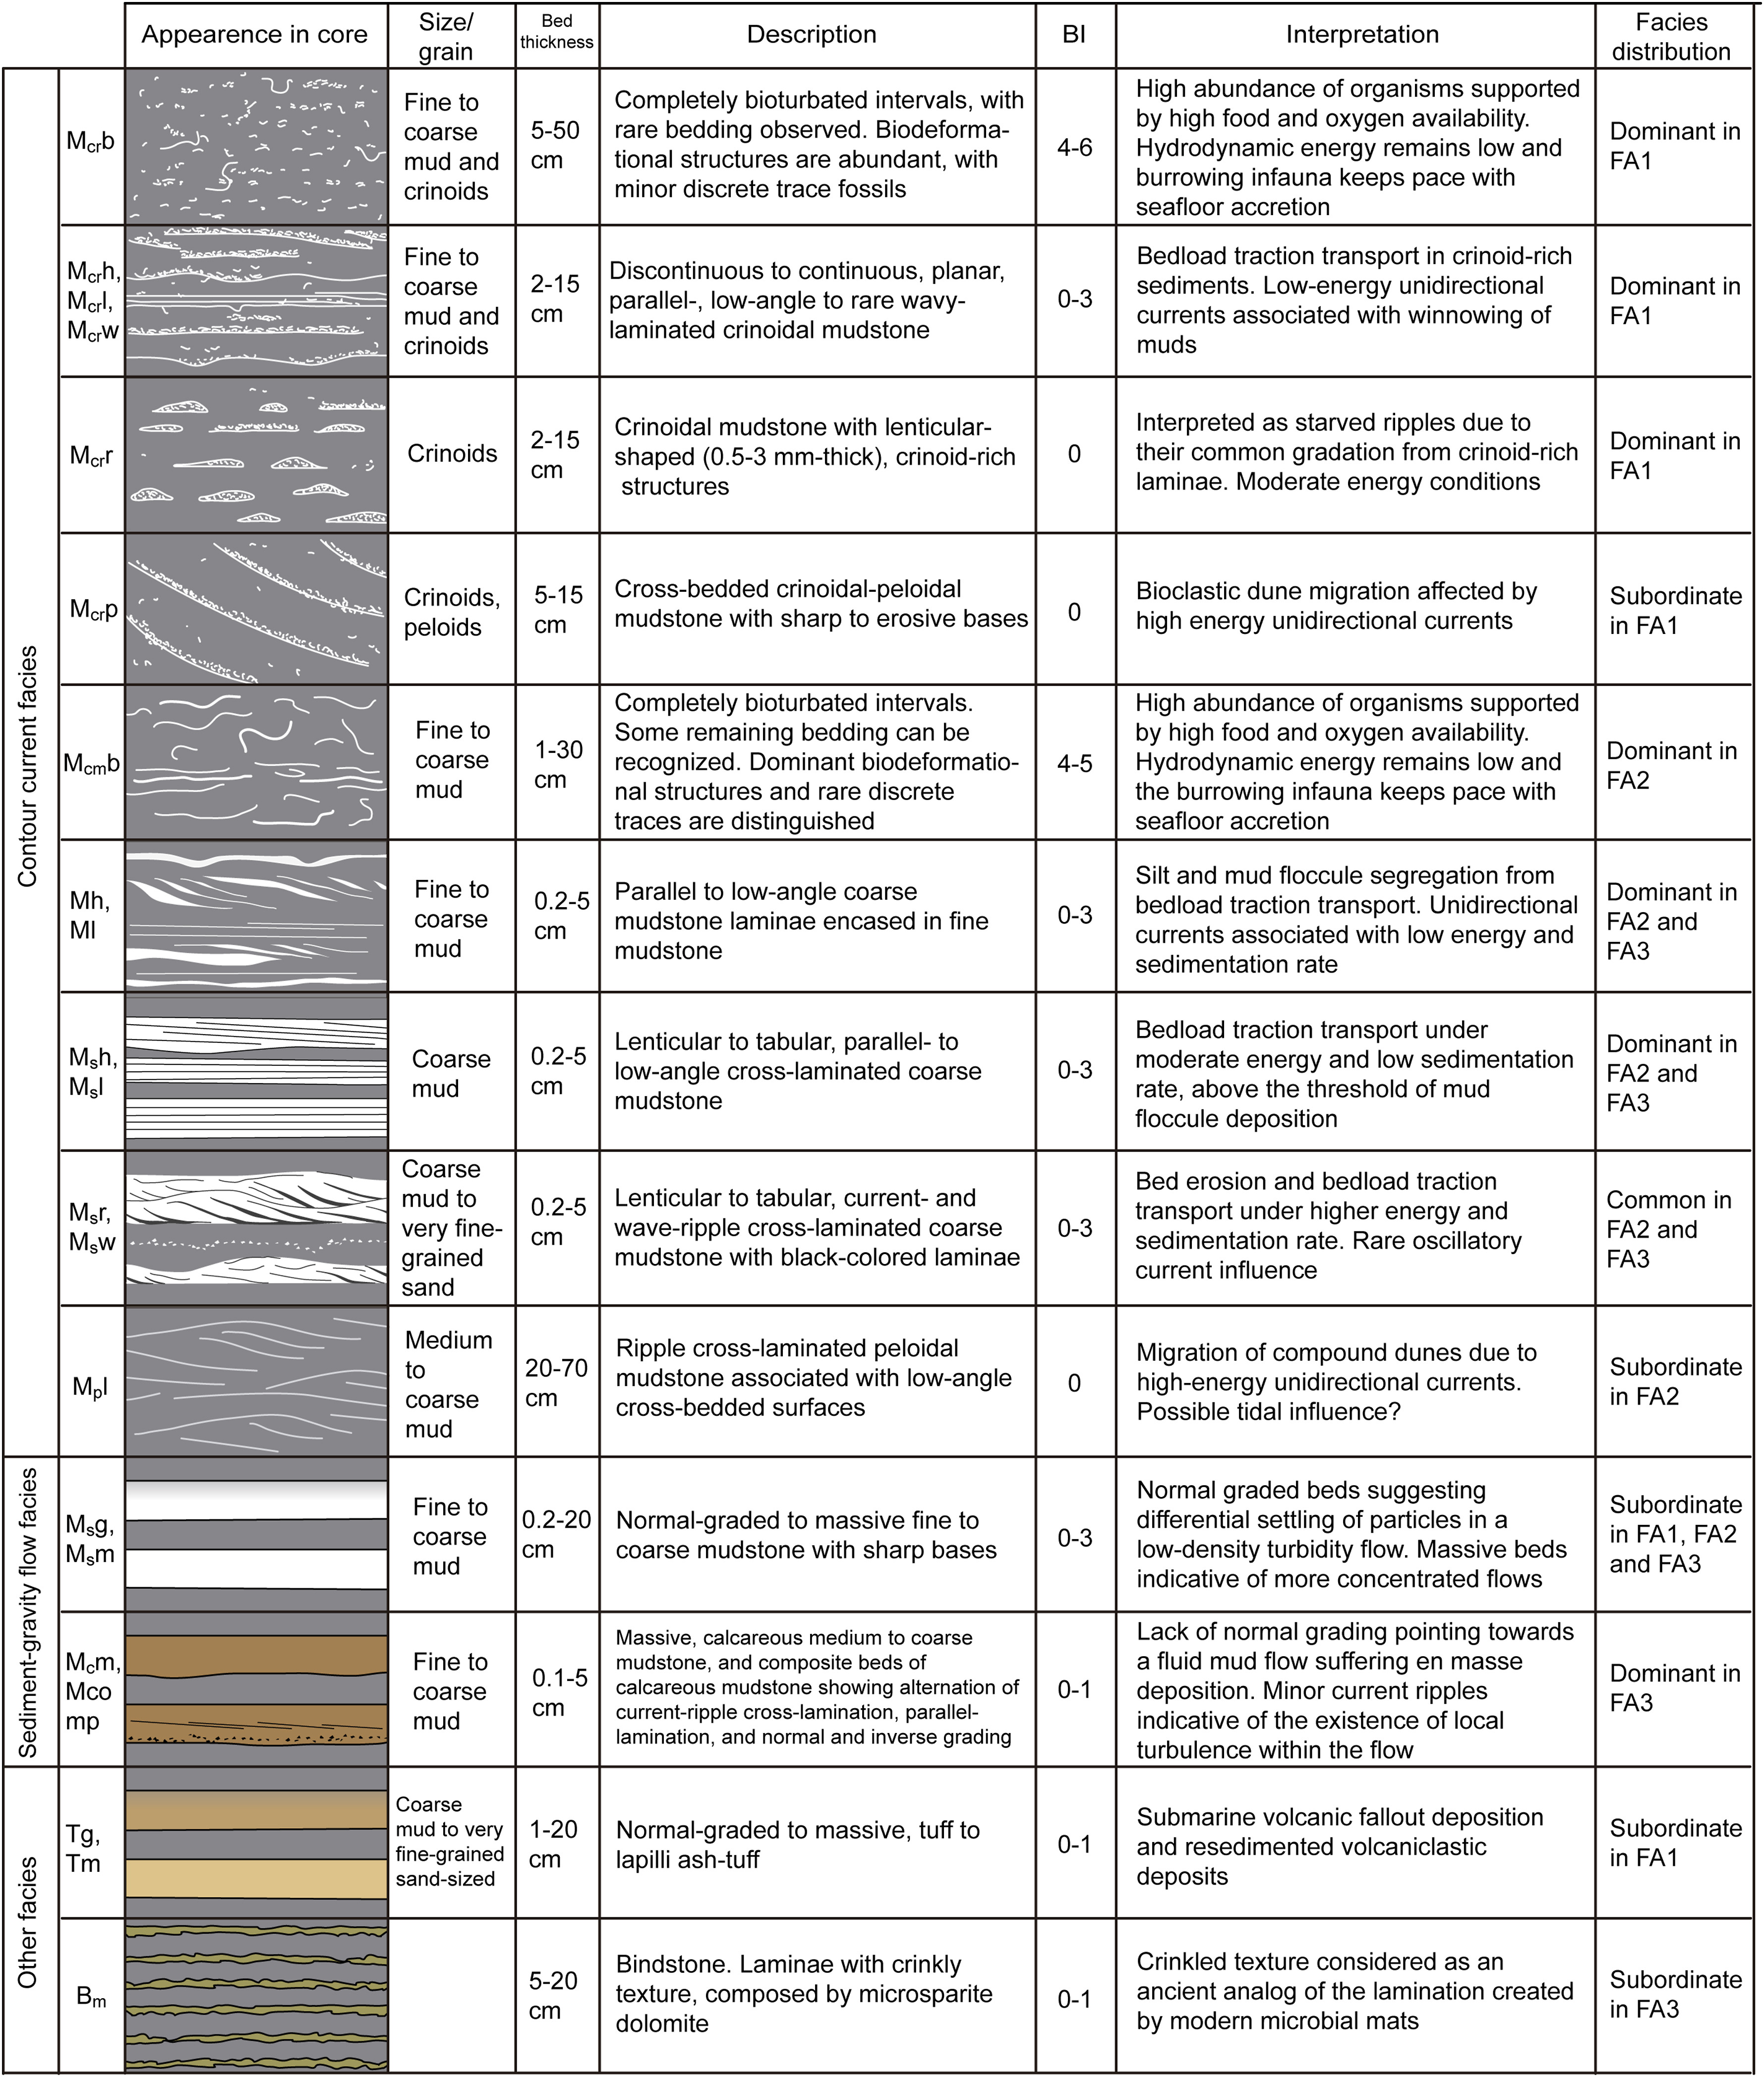
\includegraphics[width=0.75\linewidth]{Figures/0.4Field/Paz2022.jpg}
    \caption[Contourite drift facies]{Contourite drift facies \citep{Paz2022}. \textbf{Keywords:} Discontinuous, continuous, planar, parallel, low-angle, wavy pattern, lenticular shape, cross-bedding, erosional surface, tabular, cross-lamination.}
    \label{fig:Paz2022-1}
\end{figure}

\begin{figure}[h!]
    \centering
    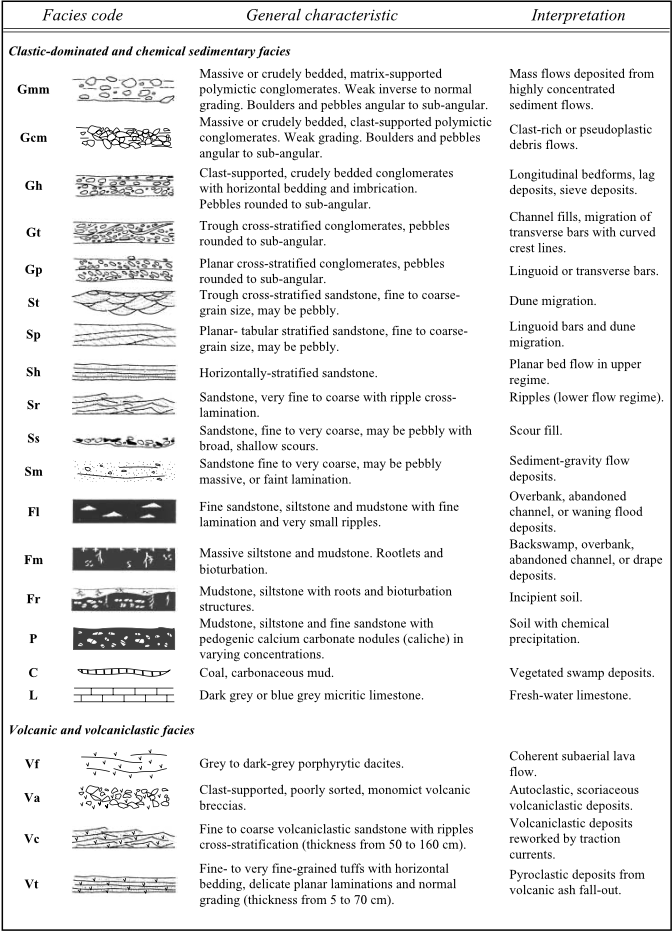
\includegraphics[width=0.75\linewidth]{Figures/0.4Field/Capuzzo2004-1.png}
    \caption[Facies description and classification in the Salvan-Dorénaz Basin]{Facies description and classification in the Salvan-Dorénaz Basin \citep{Capuzzo2004}.\textbf{Keywords:} Horizontal bedding, cross-stratification, planar, tabular, shallow scours, ripples, lamination.}
    \label{fig:Capuzzo2004-1}
\end{figure}
\clearpage